\documentclass[10pt,a4paper]{article}
\usepackage{amsmath}
\usepackage{amssymb}
\usepackage{graphicx}
\usepackage{color}
\usepackage{fancyhdr}
\usepackage{fancyvrb}
\usepackage[margin=3.5cm]{geometry}
\usepackage{framed}
\usepackage{enumerate}
\usepackage{textcomp}
\def\ket#1{\left|#1\right\rangle}
\def\bra#1{\left\langle#1\right|}
\def\braket#1{\left\langle#1\right\rangle}

\definecolor{linkcol}{rgb}{0.0, 0.0, 0.5}
\usepackage[colorlinks=true,urlcolor=linkcol,citecolor=black,linkcolor=linkcol]{hyperref}

\setcounter{section}{2}
\renewcommand\thesection{\arabic{section}}
\renewcommand\thesubsection{\thesection.\arabic{subsection}}

\fancyhf{}
\lhead{\tiny Y.~D.~Chong (2018)}
\rhead{\scriptsize MH2801: Complex Methods for the Sciences}
\lfoot{}
\rfoot{\thepage}
\pagestyle{fancy}

\makeatletter
\def\PY@reset{\let\PY@it=\relax \let\PY@bf=\relax%
    \let\PY@ul=\relax \let\PY@tc=\relax%
    \let\PY@bc=\relax \let\PY@ff=\relax}
\def\PY@tok#1{\csname PY@tok@#1\endcsname}
\def\PY@toks#1+{\ifx\relax#1\empty\else%
    \PY@tok{#1}\expandafter\PY@toks\fi}
\def\PY@do#1{\PY@bc{\PY@tc{\PY@ul
\def\PYZdl{\char`\$}
\def\PYZhy{\char`\-}
\def\PYZsq{\char`\'}
\def\PYZdq{\char`\"}
\def\PYZti{\char`\~}

\begin{document}
\setcounter{page}{19}
    
\section{Complex Numbers}\label{complex-numbers}

The \textbf{imaginary unit}, denoted $i$, is a hypothetical solution
to the quadratic equation
\begin{equation}
z^2 + 1 = 0,
\end{equation}
which is an equation that lacks real solutions. In other words,
$i = \sqrt{-1}$.

We can let the imaginary unit take part in the usual arithmetic
operations of addition and multiplication, treating it as an algebraic
quantity on the same footing as the more familiar real numbers. Thus, we
deal with numbers containing both real and imaginary parts, called
\textbf{complex numbers}. It is one of the most profound discoveries of
mathematics that this seemingly arbitrary idea gives rise to powerful
computational methods with applications in numerous fields.

    \hypertarget{complex-algebra}{%
\subsection{Complex algebra}\label{complex-algebra}}

For any complex number $z$, we can write
\begin{equation}
z = x + i y,
\end{equation}
where $x$ and $y$ are real numbers that depend uniquely on $z$. We
call these the \textbf{real part} of $z$ and the \textbf{imaginary
  part} of $z$, respectively. These real and imaginary parts are also
commonly denoted as $\mathrm{Re}(z)$ and $\mathrm{Im}(z)$, where the
$\mathrm{Re}$ and $\mathrm{Im}$ operations can be regarded as
functions mapping complex numbers to real numbers.

The set of complex numbers is denoted by $\mathbb{C}$. We can define
algebraic operations on complex numbers---addition/subtraction,
products, and taking powers---simply by following the usual rules of
algebra and setting $i^2 = -1$ whenever it shows up.

\begin{framed} \noindent
\textit{Example}---Let $z = x + i y$, where $x, y \in \mathbb{R}$. What is
$z^2$?
\begin{align*}
  z^2 &= (x+iy)^2 \\&= x^2 + 2x(iy) + (iy)^2 \\&= x^2 - y^2 + 2ixy
\end{align*}
  Hence, the real and imaginary parts are:
  \begin{equation*}
    \mathrm{Re}(z^2) = x^2 -y^2, \;\;\; \mathrm{Im}(z^2) = 2xy.
  \end{equation*}
\end{framed}

A caveat: for now, we'll only consider taking \emph{integer} powers,
such as $z^{-1}$ or $z^2$. Taking non-integer powers, such as
$z^{1/3}$, introduces vexatious complications which we'll postpone for
now (they will be dealt with when we discuss branch points and branch
cuts).

Another interesting fact, which can be easily proven, is that real
coefficients (and \emph{only} real coefficients) can be freely moved
into or out of $\textrm{Re}(\cdots)$ and $\textrm{Im}(\cdots)$
operations:
\begin{equation}
\left\{\begin{array}{l}\mathrm{Re}(\alpha z + \beta z') = \alpha \, \mathrm{Re}(z) + \beta\, \mathrm{Re}(z')\\ \mathrm{Im}(\alpha z + \beta z') = \alpha \, \mathrm{Im}(z) + \beta\, \mathrm{Im}(z')\end{array}\right.\qquad\mathrm{for}\;\alpha, \beta \in \mathbb{R}.
\end{equation}
One important consequence is that if we have a complex function of a
real variable, then we can calculate the derivative of that function
from the derivatives of the real and imaginary parts. This is shown in
the following example:

\begin{framed} \noindent
  \textit{Example}---If $z(t)$ is a complex function of a real input $t$, then
  \begin{equation}
    \mathrm{Re}\left[\frac{dz}{dt}\right] = \frac{d}{dt} \mathrm{Re}\left[z(t)\right], \;\;\textrm{and}\;\;\; \mathrm{Im}\left[\frac{dz}{dt}\right] = \frac{d}{dt} \mathrm{Im}\left[z(t)\right].
  \end{equation}
This can be proven using the definition of the derivative:
\begin{align*}
  \mathrm{Re}\left[\frac{dz}{dt}\right] &= \;\; \mathrm{Re}\left[\lim_{\delta t \rightarrow 0} \frac{z(t+\delta t) - z(t)}{\delta t}\right] \\&= \lim_{\delta t \rightarrow 0} \left[\frac{\mathrm{Re}[z(t+\delta t)] - \mathrm{Re}[z(t)]}{\delta t}\right] \\&= \frac{d}{dt} \mathrm{Re}\left[z(t)\right].
\end{align*}
The $\mathrm{Im}[\cdots]$ case works out similarly. Note that the
infinitesimal quantity $\delta t$ is real; otherwise, this wouldn't
work.
\end{framed}

\subsection{Conjugates and Magnitudes}
\label{conjugates-and-magnitudes}

For each complex number $z = x + iy$, we define its \textbf{complex
conjugate} as a complex number whose imaginary part has its sign
flipped:
\begin{equation}
z^* = x - i y.
\end{equation}
We can show that conjugation obeys two important properties:
\begin{equation}
\begin{aligned}(z_1 + z_2)^* &= z_1^* + z_2^* \\ (z_1 z_2)^* &= z_1^* z_2^*.\end{aligned}
\end{equation}

\begin{framed} \noindent
\textit{Example}---Let us prove that $(z_1 z_2)^* = z_1^* z_2^*$. First, let
$z_1 = x_1 + i y_1$ and $z_2 = x_2 + i y_2$.
Then,
\begin{align*}(z_1 z_2)^* &= \left[(x_1+iy_1)(x_2+iy_2)\right]^* \\ &= \left[\left(x_1 x_2 - y_1 y_2\right) + i\left(x_1y_2+y_1x_2\right)\right]^* \\ &= \left(x_1 x_2 - y_1 y_2\right) - i\left(x_1y_2+y_1x_2\right) \\ &= \left(x_1 - i y_1\right)\left(x_2 - i y_2\right) \\&= z_1^* z_2^*. \end{align*}
\end{framed}

For a complex number $z = x + i y$, the \textbf{magnitude} of the
complex number is
\begin{equation}
|z| = \sqrt{x^2 + y^2}.
\end{equation}
This is a non-negative real number. A complex number and its conjugate
have the same magnitude: $|z| = |z^*|$. Also, we can show that complex
magnitudes have the property
\begin{equation}
|z_1 z_2| = |z_1| \, |z_2|.
\end{equation}
This property is similar to the ``absolute value'' operation for real
numbers, hence the similar notation. As a corollary, we can show that
taking a power of a complex number raises its magnitude by the same
power:
\begin{equation}
|z^n| = |z|^n \;\;\;\textrm{for}\;\;n \in \mathbb{Z}.
\end{equation}

\subsection{Euler's formula}\label{eulers-formula}

Euler's formula is an extremely important result which states that

\begin{framed}
  \begin{equation}
    e^{iz} = \cos(z) + i \sin(z).
  \end{equation}
\end{framed}

This can be proven using the series definition of the exponential
function, which is
\begin{equation}
\exp(z) = 1 + z + \frac{z^2}{2!} + \frac{z^3}{3!} + \frac{z^4}{4!} + \frac{z^5}{5!} + \frac{z^6}{6!} + \cdots
\end{equation}
Previously, we assumed that the input to the exponential function was a
real number. However, since complex numbers can be added and multiplied
using the same rules of algebra as real numbers, we can employ this
series formula as the definition of the \textbf{complex exponential
function}. This is a function that takes complex inputs and gives
complex outputs. When the input happens to be real, the complex
exponential function gives the same output as the real exponential
function.

Plugging $iz$ as the input to the complex exponential function gives
\begin{align}
  \exp(iz) &= 1 + (iz) + \frac{(iz)^2}{2!} + \frac{(iz)^3}{3!} + \frac{(iz)^4}{4!} + \frac{(iz)^5}{5!} + \frac{(iz)^6}{6!} + \cdots \\&= 1 + iz - \frac{z^2}{2!} - i \frac{z^3}{3!} + \frac{z^4}{4!} + i \frac{z^5}{5!} - \frac{z^6}{6!} + \cdots \\& = \left(1 - \frac{z^2}{2!} + \frac{z^4}{4!} - \frac{z^6}{6!} + \cdots\right) + i\left(z  - \frac{z^3}{3!}  + \frac{z^5}{5!}  - \frac{z^7}{7!} + \cdots\right).
\end{align}
Now, compare the two terms in parentheses to the series expansions for
the cosine and sine functions. We can define the \textbf{complex
  cosine} and \textbf{complex sine} functions using these complex
series formulas:
\begin{equation}
\begin{aligned}\cos(z) &= 1 - \frac{z^2}{2!} + \frac{z^4}{4!} - \frac{z^6}{6!} + \cdots \\ \sin(z) &= z - \frac{z^3}{3!} + \frac{z^5}{5!} - \frac{z^7}{7!} + \cdots\end{aligned}
\end{equation}
These are perfect matches for the two terms in the series expansion of
the complex exponential! Hence, Euler's formula immediately follows:
\begin{equation}
e^{iz} = \cos(z) + i \sin(z).
\end{equation}
One important consequence of Euler's formula is that
\begin{equation}
\left|e^{i\theta}\right| = \sqrt{\cos^2(\theta) + \sin^2(\theta)} = 1 \qquad \mathrm{for}\; \theta \in \mathbb{R}.
\end{equation}
Another interesting consequence is that
\begin{equation}
e^{i\pi} = -1,
\end{equation}
which is a formula that relates two transcendental constants $e =
2.7182818285\dots$ and $\pi = 3.141592654\dots$, by means of the
imaginary unit. (We previously saw a different relationship between
these two constants when solving the Gaussian integral.)


\subsection{The complex plane}\label{the-complex-plane}

A convenient device for conceptualizing complex numbers is to think of a
complex number as a point on a two-dimensional plane, called the
\textbf{complex plane}. The real and imaginary parts are the horizontal
and vertical Cartesian coordinates in the plane. The horizontal ($x$)
and vertical ($y$) coordinate axes are called the ``real axis'' and
the ``imaginary axis'', respectively.

\begin{figure}[h]
  \centering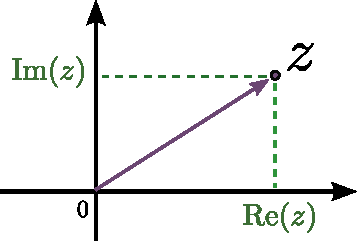
\includegraphics[width=0.32\textwidth]{complex_plane}
\end{figure}

\hypertarget{polar-representation}{%
\subsubsection{Polar representation}\label{polar-representation}}

If we think of a complex number as a point on the complex plane, its
position can also be represented using polar coordinates instead of
Cartesian coordinates. For a complex number $z = x + i y$, we can
introduce polar coordinates $r$ and $\theta$ (both real numbers),
such that
\begin{equation}
r = \sqrt{x^2 + y^2}, \;\;\; \theta = \tan^{-1}(y/x).
\end{equation}
Conversely,
\begin{equation}
x = r\cos\theta, \;\;\; y = r\sin\theta.
\end{equation}
These are the usual formulas for performing a change of coordinate
between two-dimensional Cartesian coordinates and polar coordinates,
as shown below:

\begin{figure}[h]
  \centering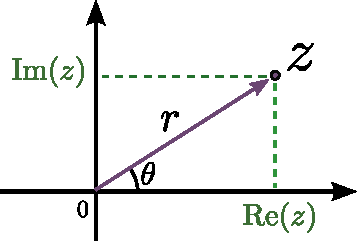
\includegraphics[width=0.32\textwidth]{complex_plane2}
\end{figure}

\noindent
The radial coordinate, $r$, is equal to what we previously defined as
the magnitude of the complex number: $r = |z|$ (see
Section~\ref{conjugates-and-magnitudes}). The azimuthal coordinate
$\theta$ is called the \textbf{argument} of the complex number, which
we sometimes denote by $\mathrm{arg}(z)$.

Using Euler's formula, we can write
\begin{align}
  z &= r\cos(\theta) + i r\sin(\theta)\\&= r \left[\cos(\theta) + i \sin(\theta)\right] \\&= r \, e^{i\theta}.
\end{align}
This tells us that whenever we can manipulate a complex number into a
form $A e^{iB}$, where $A$ and $B$ are real numbers, then $A$ is
the magnitude and $B$ is the argument. This is used in the following
example:

\begin{framed} \noindent
\textit{Example}---For $z \in \mathbb{C}$, it can be shown that the
magnitude and argument of $\exp(z)$ are:
\begin{equation}
  \displaystyle\left|\exp(z)\right| = e^{\mathrm{Re}(z)}, \quad \mathrm{arg}\left[\exp(z)\right] = \mathrm{Im}(z).
\end{equation}
Proof: Let $z = x + i y$, where $x, y \in \mathbb{R}$; then
\begin{equation}
  e^{z} = e^{x + i y} = e^x \, e^{iy}.
\end{equation}
By inspection, the magnitude of this complex number is $e^x$, and its
argument is $y$.
\end{framed}

Note, by the way, that the complex number zero, $z = 0$, has zero
magnitude and \emph{undefined} argument.

\subsubsection{Geometrical interpretation of complex operations}
\label{geometrical-interpretation-of-complex-operations}

Using the complex plane, we can give useful geometric interpretations to
the basic operations on complex numbers:

\begin{itemize}
\item 
Addition of two complex numbers can be interpreted as the addition of
two coordinate vectors. If $z_1 = x_1 + i y_1$ and $z_2 = x_2 + i
y_2$, then
\begin{equation}
  z_1 + z_2 = \left(x_1 + x_2\right) + i\left(y_1 + y_2\right).
\end{equation}
Hence, the point corresponding to $z_1 + z_2$ is obtained by adding
the two coordinate vectors corresponding to $z_1$ and $z_2$. From
this, we can geometrically prove a useful inequality relation between
complex numbers, called the ``triangle inequality'':
\begin{equation}
  |z_1 + z_2| \le |z_1| + |z_2|.
\end{equation}

\item
Complex multiplication can be interpreted as a scaling together with a
rotation. If $z_1 = r_1e^{i\theta_1}$ and $z_2 = r_2e^{i\theta_2}$,
then
\begin{equation}
  z_1 z_2 = \left(r_1 r_2\right) \,\exp[i(\theta_1 + \theta_2)].
\end{equation}
Hence, the point corresponding to $z_1 \, z_2$ is obtained by scaling
the $z_1$ coordinate vector by a factor of $|z_2|$, and rotating it by
an angle of $\theta_2$ around the origin. In particular,
multiplication by $e^{i\theta}$ is equivalent to a pure rotation of
angle $\theta$.

\item
  Complex conjugation (Section~\ref{conjugates-and-magnitudes}) is
  equivalent to reflection about the real axis.  It moves a point from
  the upper half of the complex plane to the lower half, or vice
  versa.
\end{itemize}

\subsubsection{Complex numbers have no ordering}
\label{complex-numbers-have-no-ordering}

One consequence of the fact that complex numbers reside in a
two-dimensional plane is that \emph{inequality relations are not
  defined for complex numbers}. This is one important difference
between complex numbers and real numbers.

Real numbers can be \textbf{ordered}, which means that for any two real
numbers $a$ and $b$, one and only one of the following is true:
\begin{equation}
a < b \;\; \mathrm{OR} \;\; a = b \;\; \mathrm{OR}\;\; a > b.
\end{equation}
In geometrical terms, these ordering relations exist because the real
numbers reside along a one-dimensional line.

But because complex numbers lie in a two-dimensional plane, it is
nonsensical to write something like $z_1 < z_2$, where $z_1$ and
$z_2$ are complex numbers. (It is, however, valid to write
$|z_1| < |z_2|$, since magnitudes are real.)

\subsection{Complex functions}\label{complex-functions}

When deriving Euler's formula in Section~\ref{eulers-formula}, we
introduced \textbf{complex functions} that were defined by taking real
mathematical functions, like the exponential, and making them accept
complex number inputs. Let us take a closer look at how these complex
functions behave.

\subsubsection{Complex trigonometric functions}
\label{complex-trigonometric-functions}

The complex sine and cosine functions are defined using the same
series expansions as the real cosine and sine functions, except that
the inputs $z$ are allowed to be complex:
\begin{align}
  \sin(z) = z - \frac{z^3}{3!} + \frac{z^5}{5!} - \frac{z^7}{7!} + \cdots \\
  \cos(z) = 1 - \frac{z^2}{2!} + \frac{z^4}{4!} - \frac{z^6}{6!} + \cdots
\end{align}
It is important to note that the \emph{outputs} of the complex
trigonometric functions are complex numbers too. Therefore, some of
the familiar properties of the real trigonometric functions don't
apply. For instance, $|\sin(z)|$ and $|\cos(z)|$ are \emph{not}
bounded by 1 when $z$ is not real.
            
We can also write the complex cosine and sine functions in terms of
the exponential:
\begin{align}
  \cos(z) &= \;\;\frac{1}{2}\left(e^{iz} + e^{-iz}\right) \label{cosz}\\
  \sin(z) &= -\frac{i}{2}\left(e^{iz} - e^{-iz}\right). \label{sinz}
\end{align}

This is often a convenient step when solving integrals, as shown in
the following example:

\begin{framed} \noindent
  \textit{Example}---Consider the (real) integral
\begin{equation*}
  I = \int_0^\infty dx \; e^{- x} \, \cos(x).
\end{equation*}
One way to solve this is to use integration by parts, but another way
is to use the complex expansion of the cosine
function:
\begin{align*}
  I &= \int_0^\infty dx \; e^{- x}
\,\frac{1}{2}\, \left[e^{ix} + e^{-ix}\right] \\ &= \frac{1}{2}
\int_0^\infty dx \; \left[e^{(-1+i)x} + e^{(-1-i)x}\right] \\ &=
\frac{1}{2} \left[ \frac{e^{(-1+i) x}}{-1+i} + \frac{e^{(-1 - i)
      x}}{-1 - i}\right]_0^\infty \\ &= -\frac{1}{2}
\left(\frac{1}{-1+i} + \frac{1}{-1 - i}\right) \\ &=
\frac{1}{2}.
\end{align*}
\end{framed}
     
\subsubsection{Complex trigonometric identities}

Euler's formula provides a convenient way to deal with trigonometric
functions. Consider the addition formulas
\begin{align}
  \sin(z_1 + z_2) &= \sin(z_1) \cos(z_2) + \cos(z_1)\sin(z_2) \\
  \cos(z_1 + z_2) &= \cos(z_1) \cos(z_2) - \sin(z_1)\sin(z_2).
\end{align}
As discussed in Chapter 0, the standard proofs for these formulas are
geometric: you draw a figure, and solve a bunch of relations between
the angles and sides of the various triangles, making use of the
Pythagorean formula. But using the Euler formula, we can prove these
algebraically. For example,
\begin{align}
  \cos(z_1)\cos(z_2) &= \frac{1}{4}\left(e^{iz_1} + e^{-iz_1}\right) \left(e^{iz_2} + e^{-iz_1}\right)\\&= \frac{1}{4}\left[e^{i(z_1+z_2)} + e^{i(-z_1 + z_2)} + e^{i(z_1 -z_2)} + e^{-i(z_1+z_2)}\right] \\ \sin(z_1)\sin(z_2) &= -\frac{1}{4}\left(e^{iz_1} - e^{-iz_1}\right) \left(e^{iz_2} - e^{-iz_1}\right) \\ &= -\frac{1}{4}\left[e^{i(z_1+z_2)} - e^{i(-z_1 + z_2)} - e^{i(z_1 -z_2)} + e^{-i(z_1+z_2)}\right].
\end{align}
Thus,
\begin{equation}
  \cos(z_1) \cos(z_2) - \sin(z_1)\sin(z_2) = \frac{1}{2}\left[e^{i(z_1+z_2)} + e^{-i(z_1+z_2)}\right] = \cos(z_1 + z_2).
\end{equation}
As a bonus, these addition formulas now hold for complex inputs as well,
not just real inputs.

\subsubsection{Hyperbolic functions}
\label{hyperbolic-functions}

Euler's formula also provides us with a link between the trionometric
and hyperbolic functions. From the definition of the hyperbolic
functions:
\begin{equation}
\sinh(z) = \frac{1}{2}\left(e^{z} - e^{-z}\right), \quad\; \cosh(z) = \frac{1}{2}\left(e^{z} + e^{-z}\right)
\end{equation}
Comparing this to Eqs.~\eqref{cosz} and \eqref{sinz}, we can see that
the trigonometric and hyperbolic functions are related by
\begin{align}
  \begin{aligned}
    \sin(z) &= -i \sinh(iz), \quad \cos(z) = \cosh(iz) \\
    \sinh(z) &= -i \sin(iz), \quad \cosh(z) = \cos(iz)
  \end{aligned}
\end{align}
Using these relations, we can relate the addition formulas for
trignometric formulas to the addition formulas for hyperbolic functions,
e.g.
\begin{align}
  \cosh(z_1+z_2) &= \cos(iz_1 + iz_2) \\
  &= \cos(iz_1)\cos(iz_2) - \sin(iz_1)\sin(iz_2) \\
  &= \cosh(z_1)\cosh(z_2) + \sinh(z_1)\sinh(z_2).
\end{align}

\subsection{Trajectories in the complex plane}
\label{trajectories-in-the-complex-plane}

If we have a function $z(t)$ which takes a real input $t$ and outputs
a complex number $z$, it is often useful to plot a curve in the
complex plane called the ``parametric trajectory'' of $z$. Each point
on this curve indicates the value of $z$ for a particular value of
$t$. We will give a few examples below.

First, consider
\begin{equation}
z(t) = e^{i\omega t}, \quad \omega \in \mathbb{R}.
\end{equation}
The trajectory is a circle in the complex plane, centered at the origin
and with radius 1:

\begin{figure}[h]
  \centering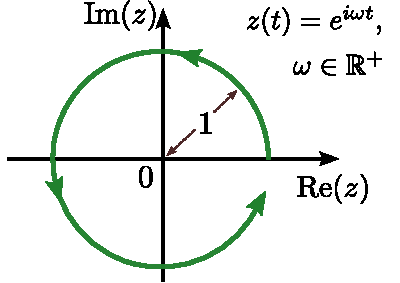
\includegraphics[width=0.37\textwidth]{complex_trajectory_1}
\end{figure}

To see why, observe that the function has the form $z(t) =
r(t)\,e^{i\theta(t)}$, which has magnitude $r(t) = 1$, and argument
$\theta(t) = \omega t$ varying proportionally with $t$. If $\omega$ is
positive, the argument increases with $t$, so the trajectory is
counter-clockwise; if $\omega$ is negative, the trajectory is
clockwise.

Next, consider
\begin{equation}
z(t) = e^{(\gamma + i \omega) t},
\end{equation}
where $\gamma,\omega \in \mathbb{R}.$ For $\gamma = 0$, this reduces
to the previous example. For $\gamma \ne 0$, the trajectory is a
spiral:

\begin{figure}[h]
  \centering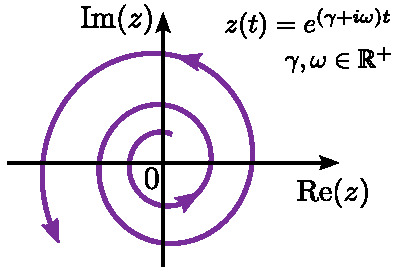
\includegraphics[width=0.37\textwidth]{complex_trajectory_2}
\end{figure}

To see this, we again observe that this function can be written in the
form
\begin{equation}
z(t) = r(t) \;e^{i\theta(t)},
\end{equation}
where $r(t) = e^{\gamma t}$ and $\theta = \omega t.$ The argument
varies proportionally with $t$, so the trajectory loops around the
origin. The magnitude increases with $t$ if $\gamma$ is positive, and
decreases with $t$ if $\gamma$ is negative. Thus, for instance, if
$\gamma$ and $\omega$ are both positive, then the trajectory is an
anticlockwise spiral moving outwards from the origin.

Finally, consider
\begin{equation}
z(t) = \frac{1}{\alpha t + i\beta}.
\end{equation}
This trajectory is a circle which passes through the origin, as shown
below:

\begin{figure}[h]
  \centering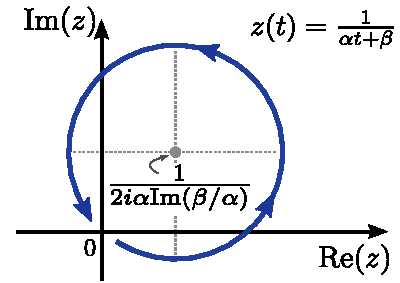
\includegraphics[width=0.37\textwidth]{complex_trajectory_3}
\end{figure}

\noindent
Proving this requires a bit of ingenuity, and is left as an
exercise. (This is an example of something called a
\href{http://en.wikipedia.org/wiki/M\%C3\%B6bius_transformation}{Möbius
  transformation}.)

\subsection{Why complex numbers?}
\label{why-complex-numbers}

Here are a couple of questions that might have occurred to you:

\begin{itemize}
\item
  Integers and real numbers have intuitive connections to the phenomena
  we experience in everyday life, such as the counting of discrete
  objects, or measuring lengths and weights. Complex numbers, however,
  seem like completely abstract concepts. Why should we study them?
\item
  If we extend the concept of numbers to complex numbers, why stop here?
  Why not extend the concept further, and formulate other abstract
  number systems that are even more complicated than complex numbers?
\end{itemize}

Let's try to address the second question first. Recall our earlier
observation that complex numbers can be manipulated via the same rules
of algebra as real numbers: we can use them to add, subtract,
multiply, and divide (apart from division by zero), without running
into any logical inconsistencies. As discussed in
Section~\ref{complex-numbers-have-no-ordering}, however, complex
numbers cannot be ordered, so complex algebra can only handle
equations, not inequality relations.

On the other hand, there is one very important feature possessed by
complex numbers and not real numbers: the complex numbers are
\emph{algebraically closed}. This means that all complex polynomial
equations have solutions in $\mathbb{C}$. The set of real numbers,
$\mathbb{R}$, lacks this property: there are certain real algebraic
equations we can write down, like $x^2 + 1 = 0$, which have no
solution in $\mathbb{R}$. The ``closure'' property of $\mathbb{C}$
is called the
\href{https://en.wikipedia.org/wiki/Fundamental_theorem_of_algebra}{Fundamental
Theorem of Algebra}, which gives an idea of its importance. One
consequence of the theorem is that $\mathbb{C}$ cannot be generalized
to a more complicated number system via the same route used to extend
$\mathbb{R}$ into $\mathbb{C}$.

There do exist number systems more complicated than the complex numbers,
which are formulated not by algebraic extension, but by discarding one
or more of the rules of algebra. The
\href{https://en.wikipedia.org/wiki/Quaternion}{quaternions} are a
system of four-component numbers which obey an algebra that is
\emph{non-commutative} (i.e., $ab = ba$ is not generally true). The
\href{https://en.wikipedia.org/wiki/Octonion}{octonions} are an even
more complicated system of eight-component numbers which are not only
non-commutative but also non-associative (i.e., $(ab)c = a(bc)$ is not
generally true). These and other still-more-complicated number systems
have a few applications in physics and other fields, but are overall
much less important than $\mathbb{C}$.

One big reason that complex numbers are so important and useful is
that it's easy to formulate a version of calculus for them. The study
of smooth complex functions, and their derivatives and integrals, is
called \textbf{complex analysis}. This is a subject that we will
discuss extensively in this course.  We will see that it has important
implications for the \emph{real} calculus; for example, many real
integrals can be easily solved by first generalizing them into complex
integrals. By contrast, since quaternions and octonions are not
commutative, the concept of ``derivative'' becomes tricky to define
for these number systems, which makes it harder to formulate a useful
calculus.

     
\subsection{Exercises}

\begin{enumerate}
\item
  Let $z = x + iy$, where $x, y \in \mathbb{R}$. For each of the
  following expressions, find (i) the real part, (ii) the imaginary
  part, (iii) the magnitude, and (iv) the complex argument, in terms
  of $x$ and $y$:
  \begin{enumerate}
  \item $z^2$
  \item $1/z$
  \item $\exp(z)$
  \item $\exp(iz)$
  \item $\cos(z)$
  \end{enumerate}
  
\item
  Show that $|z_1 z_2| = |z_1|\, |z_2|$, by using (i) the polar
  representation, and (ii) the Cartesian representation.

\item
  Show that $(z_1 z_2)^* = z_1^* z_2^*$, by using (i) the polar
  representation, and (ii) the Cartesian representation.

\item Identify the problem with this chain of equations:
  \begin{equation*}
    -1 = i \cdot i = \sqrt{-1}\,\sqrt{-1} = \sqrt{-1 \cdot -1} = \sqrt{1} = 1.
  \end{equation*}

\item With the aid of Euler's formula, prove that:
  \begin{enumerate}
  \item $\cos(3x) = 4[\cos(x)]^3 -3\cos(x)$
  \item $\sin(3x) = 3\sin(x)-4[\sin(x)]^3$
  \end{enumerate}

\item
  For $z_1, z_2 \in \mathbb{C}$ and $\theta \in \mathbb{R}$, show that
  \begin{equation}
    \mathrm{Re}\left[z_1 e^{i\theta} + z_2 e^{-i\theta}\right] = A \cos(\theta) + B \sin(\theta)
  \end{equation}
  for some $A, B \in \mathbb{R}$. Find explicit expressions for $A$
  and $B$ in terms of $z_1$ and $z_2$.

\item
  As discussed in
  Section~\ref{geometrical-interpretation-of-complex-operations}, the
  conjugation operation corresponds to a reflection about the real
  axis.  What operation corresponds to a reflection about the
  imaginary axis?

\item
  Consider the complex function of a real variable $z(t) = 1/(\alpha t
  + \beta)$, where $\alpha, \beta \in \mathbb{C}$ and $t \in
  \mathbb{R}$.
  \begin{enumerate}
  \item
  For $\alpha = 1$ and $\beta = i$, show that $z(t)$ can be
  re-expressed as $z(s) = (1+e^{is})/(2i)$, where $s \in (-\pi,\pi)$.
  Hint: find a real mapping $t(s)$.

\item
  Hence, show that the trajectory for arbitrary complex values of
  $\alpha,\, \beta$ has the form of a circle.
  \end{enumerate}

\item
  With the help of a computer plotting program, generate complex
trajectories for the following functions (for real inputs
$t \in\mathbb{R}$). Explain their key features, including the
directions of the trajectories:
\begin{enumerate}
\item
$z(t) = \left[1+\frac{\cos(\beta t)}{2}\right] \, \exp(it)$, for
$\beta = 10$ and for $\beta = \sqrt{5}$.

\item $z(t) = -it \pm \sqrt{1 - t^2}$.

\item $z(t) = ae^{it} + be^{-it}$, for $a = 1, b = -2$ and for
$a = 1, b = 2$.
\end{enumerate}
\end{enumerate}

\end{document}
